\chapter{Estudo de Caso} \label{estudodecaso}

Como foi dito na seção \ref{cap:introducao}, o problema de como realizar o
acompanhamento de métricas de vulnerabilidade de código fonte ainda não foi bem
explorado dentro do contexto da Engenharia de Software. A partir disso,
foi realizado um estudo de caso com o intuito de tentar identificar qual a melhor forma
de se acompanhar e analisar métricas de código fonte dessa natureza. O estudo
de caso realizado neste trabalho visa testar algumas hipóteses iniciais que serão apresentadas
neste mesmo capítulo, além de identificar possíveis melhorias para a continuação
do mesmo.

\section{Metodologia} \label{sec:metodologia}

A metodologia utilizada neste estudo de caso foi feita baseada no trabalho
realizado por \emph{Meirelles} (\citeyear{meirelles2013}), onde foram levantadas
hipóteses iniciais e cujo objetivo é testar tais hipóteses. A definição das
hipóteses iniciais levantadas será apresentada na subseção \ref{subsec:hipoteses}.

A fim de facilitar o entendimento das atividades realizadas neste estudo de
caso, será apresentado a seguir o processo executado. Através do
fluxograma \ref{fig:processo_estudo_de_caso} pode-se ver o sequenciamento das
atividades realizadas e logo a seguir, na lista \ref{desc_processo}, o
detalhamento de cada uma delas.

\begin{figure}[h]
  \centering
  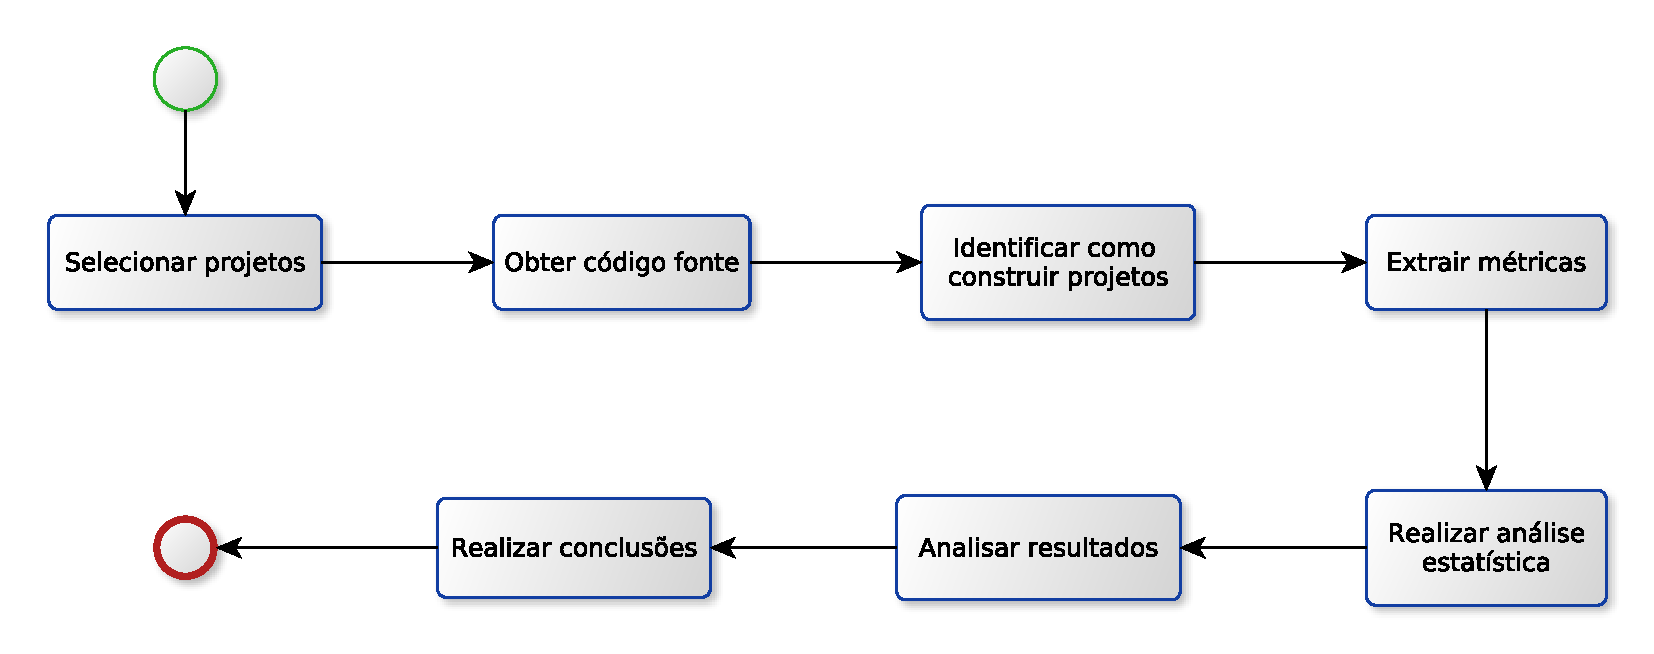
\includegraphics[width=0.9\textwidth]
      {figuras/estudo_de_caso_processo.eps}
  \caption{Processo para execução do estudo de caso}
  \label{fig:processo_estudo_de_caso}
\end{figure}

Detalhamento das atividades apresentadas no fluxograma
\ref{fig:processo_estudo_de_caso}:

\begin{enumerate}\label{desc_processo}
  \item \textbf{Selecionar projetos}: Selecionar projeto de software representativo no contexto de
    vulnerabilidades de código fonte. Foi considerado como representativo, um
    software que tenha um viés maior em segurança devido a ocorrência de ataques
    sobre o mesmo.
  \item \textbf{Obter código fonte}: Obter código fonte do projeto selecionado. Foi utilizado o código fonte
  da última versão estável do projeto.
  \item \textbf{Identificar como construir projetos}: Identificar como construir projeto selecionado. O projeto foi contruído
    segundo as orientações da própria comunidade referente ao mesmo.
  \item \textbf{Extrair métricas}: Executar ferramenta de extração de métricas de vulnerabilidade de código
    fonte. Também foram utilizadas instruções presentes na documentação da
    ferramenta em questão.
  \item \textbf{Realizar análise estatística}: Realizar análise estatísticas sobre as métricas extraídas. Foram feitos
    tratamentos necessários das informações obtidas através da análise estática
    de código fonte, já que da maneira que foi disponibilizado pela ferramenta
    não atendia os requisitos do processo de análise estatística realizado.
  \item \textbf{Analisar resultados}: Analisar resultados gerados pela análise
    estatística. Esse estudo foi uma atividade
    manual, observando os gráficos e tabelas gerados pela atividade anterior.
  \item \textbf{Realizar conclusões}: Definir se a hipótese testada estava correta ou não.
\end{enumerate}

Para a realização de algumas das atividades apresentadas foram utilizadas
ferramentas para a automação das mesmas, sendo elas:

\begin{itemize}
  \item \textit{Clang Static Analyzer}, para a extração das métricas de
    vulnerabilidade de código fonte.
  \item \textit{Scripts} para adequação do formato das métricas, servindo de
    apoio a atividade de Realizar análise estatística.
  \item \textit{Scripts} para análise estatísticas, que foram elaborados no
    trabalho de \emph{Meirelles} (\citeyear{meirelles2013})
\end{itemize}

Inicialmente o intuito era utilizar a ferramenta \emph{Analizo} para a extração
das métricas de vulnerabilidade, entretanto, foram encontradas limitações na
implementação dessa \textit{feature} e por isso foi utilizada a ferramenta
\emph{Clang Static Analyzer}. A evolução dessa funcionalidade da ferramenta
\emph{Analizo} constitui um dos objetivos deste trabalho, como foi apresentado na seção
\ref{sec:objetivos}. Atualmente, o autor deste trabalho é um dos mantenedores da
ferramenta \emph{Analizo}, e compôs a equipe de desenvolvimento da
\textit{feature} em questão.

Para o entendimento completo do estudo de caso, serão apresentadas as
ferramentas utilizadas na subseção \ref{subsec:ferramentas}, iniciando pela ferramenta \emph{Analizo}, que
não foi utilizado no estudo, mas que será alvo de uma das contribuições deste
trabalho. Em seguida, serão apresentadas a ferramenta \emph{Clang Static
Analyzer}, e os \textit{Scripts} utilizados.

O teste das hipóteses, desde a coleta dos dados até a análise dos resultados, serão
apresentados na subseção \ref{subsec:teste_hipotese}. Nessa subseção será
apresentado a corretude ou não das hipóteses.

\subsection{Hipóteses} \label{subsec:hipoteses}

As hipóteses iniciais levantadas para este estudo de caso, foram feitas baseadas em
formas de se acompanhar e analisar métricas de \textit{design} de código fonte
apresentadas em outros trabalhos, como em \emph{Meirelles}
(\citeyear{meirelles2013}). Logo, as hipóteses são:

\begin{itemize}
  \item \textit{H1}: As métricas de vulnerabilidade de código fonte podem ser
    observadas de maneira similar as métricas de \textit{design} de código
    fonte.
  \item \textit{H2}: A média dos valores das métricas de vulnerabilidade de
    código fonte, geralmente, não é representativa para o acompanhamento das mesmas.
  \item \textit{H3}: Os valores das métricas de vulnerabilidade de código fonte
    se comportam como distribuições estatísticas de cauda longa, e não
    distribuições estatísticas normalizáveis.
\end{itemize}

Todas as hipóteses apresentadas foram levantadas devido aos resultados apresentados em
\emph{Meirelles} (\citeyear{meirelles2013}), por serem satisfatórios e
considerados como premissas iniciais. Sendo validadas e confirmadas as hipóteses
acima, será possível encontrar valores de referência baseado em análises
quantitativas dos valores das métricas de vulnerabilidade. 

\subsection{Ferramentas} \label{subsec:ferramentas}

Nesta seção serão apresentadas as ferramentas utilizadas neste estudo de caso.

\subsubsection{Analizo} \label{analizo}

\emph{Analizo} é um conjunto de ferramentas livre, multilinguagem (C, C++, Java), realiza análise de código fonte, é facilmente 
extensível e disponibiliza diferentes tipos de visualização. Ele suporta a extração e cálculo de um bom número de métricas de 
código fonte, geração de gráficos de dependência e análise de evolução do software \cite{analizo}.

A seguir as funcionalidades da ferramenta \emph{Analizo} \footnote{Disponível em
\url{http://www.analizo.org/features.html}}:

\begin{itemize}
  \item Analisar código-fonte escritos em C, C ++ e Java.
  \item Extrair métricas de código-fonte.
  \item Extrair métricas de uma grande quantidade de projetos em lote (\textit{batch mode}).
  \item Extrair métricas de um repositório.
  \item Desenhar gráfico de dependências.
  \item Analisar evolução do software (analisa-se várias versões do software e uma matriz de evolução é produzida).
\end{itemize}

Será iniciado o processo de manutenção corretiva da funcionalidade de extração de métricas de vulnerabilidade de código fonte 
para as linguagens C e C++, para que melhor atenda as necessidades deste trabalho. Outra funcionalidade que ainda está em 
processo de desenvolvimento é a adição do suporte da linguagem \textit{Perl}.

A ferramenta \emph{Analizo} é facilmente extensível, desde extratores até formas
de visualizações. A figura \ref{archanalizo} mostra
como está implementada a arquitetura em camadas da ferramenta \cite{analizoartigo}. Existem basicamente cinco módulos, o 
\textit{Core} é o módulo responsável por atividades centrais como processamento,
filtros e modelos dentre outros; 
\textit{Extractor} é o módulo que contém os extratores de métricas de código
fonte utilizados, atualmente existem três: \textit{Clang}, \textit{Doxyparse}
e \textit{Sloccount}; \textit{Metrics} é o módulo que contém a lógica para
cálculo de todas as métricas, atualmente possui
37 (trinta e sete) métricas de módulo e 4 (quatro) métricas globais; \textit{Output} é o módulo que será dada a saída da 
ferramenta, atualmente existem opções de banco de dados e arquivo CSV; \textit{Tools} é o módulo que representa várias outras
ferramentas que podem trabalhar tanto acima do \textit{Core} quanto acima dos outros módulos.

\begin{figure}[h]
  \centering
  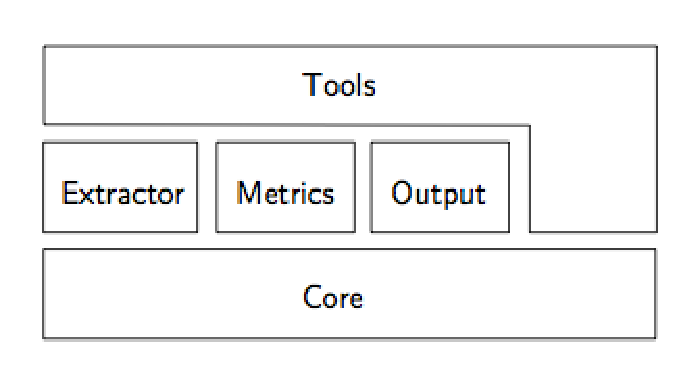
\includegraphics[width=0.4\textwidth]
      {figuras/analizo.eps}
  \caption{Arquitetura da ferramenta Analizo}
  \label{archanalizo}
\end{figure}

\subsubsection{Clang} \label{clang}

\emph{Clang} é um compilador \textit{front end} para as linguagens de
programação C, C++ e \textit{Objective-C}. O \emph{Clang} faz parte
do projeto LLVM \textit{Open Source} e utiliza o mesmo como seu \textit{backend}. 

O \emph{Clang} possui algumas funcionalidades e metas disponíveis no seu respectivo
\textit{site}\footnote{Disponível em: \url{http://clang.llvm.org}}, e
algumas das principais metas são:

\begin{itemize}
  \item Rápida compilação e baixo uso de memória
  \item Diagnóstico expressivos (exemplo, apresentar erros de uma maneira fácil para o usuário)
  \item Compatibilidade com o GCC
  \item Suportar diversos clientes (exemplo, análise estática e refatoração)
  \item Código fonte base simples e de fácil entendimento ("\textit{hackable}")
\end{itemize}

Algumas dessas metas estão sendo atingidas, por exemplo, um experimento
realizado por \emph{Naroff} (\citeyear{naroff2009}), evidenciou o rápido
tempo de compilação do \emph{Clang} em comparação com o \emph{GCC}, principal
compilador para linguagem C/C++ disponível no mercado. Foi feita a compilação do \textit{PostgreSQL} em computadores com as
mesmas configuraçãoes de \textit{hardware} e o resultado obtido é expresso pela figura \ref{clang_gcc}.

\begin{figure}[h]
  \centering
  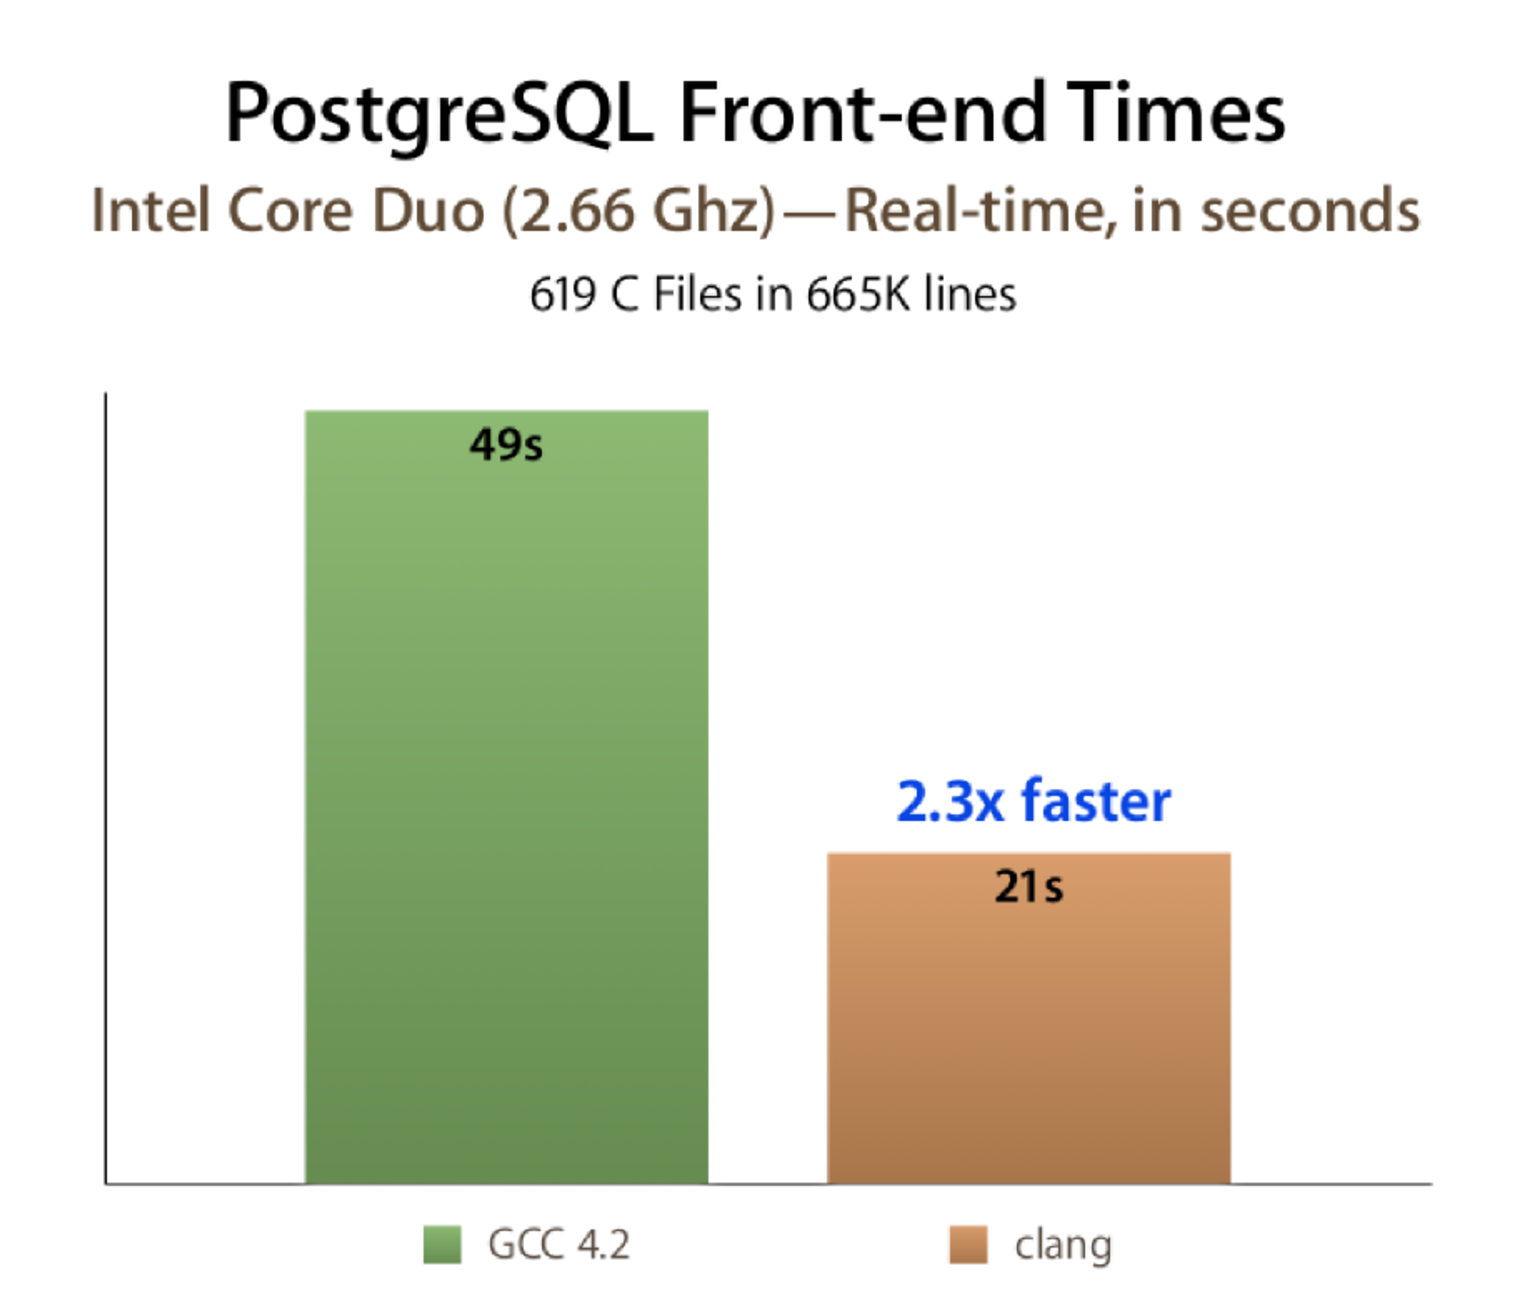
\includegraphics[width=0.4\textwidth]
      {figuras/clang_gcc.eps}
      \caption{Análise de performance do \emph{Clang} em comparação com o
      \emph{GCC}}
  \label{clang_gcc}
\end{figure}

O \emph{Clang} vem sendo desenvolvido baseado na arquitetura do projeto
\emph{LLVM}, possui bibliotecas centrais e bibliotecas de 
aplicativos, conforme é apresentado na figura \ref{clang_arch}. No contexto desse trabalho, o foco é a biblioteca de aplicativo
\textit{Analysis}. A ideia dessa biblioteca é trazer alguns benefícios para os desenvolvedores, como o descobrimento de 
\textit{bugs} o mais cedo possível; checar sistematicamente o código fonte; achar alguns \textit{bugs} mesmo na falta de caso
de testes, no caso de trechos de código difíceis de serem testados \cite{kremenek2009}. 

A análise estática realizada pelo \emph{Clang} é interprocedural, podendo achar inconsistências entre funções/métodos, para isso,
é necessária a compilação do código fonte, onde nessa fase será construída a AST 
\cite{kremenek2009}. Essa característica pode não ser muito atraente a primeira vista, pois para realizar a análise do código 
fonte é necessário compila-lo, entretanto, pode ser um ponto positivo tendo em vista que a todo momento que for feita 
construção do software a análise será realizada, mesmo que essa questão tenha sido esquecida.

\begin{figure}[h]
  \centering
  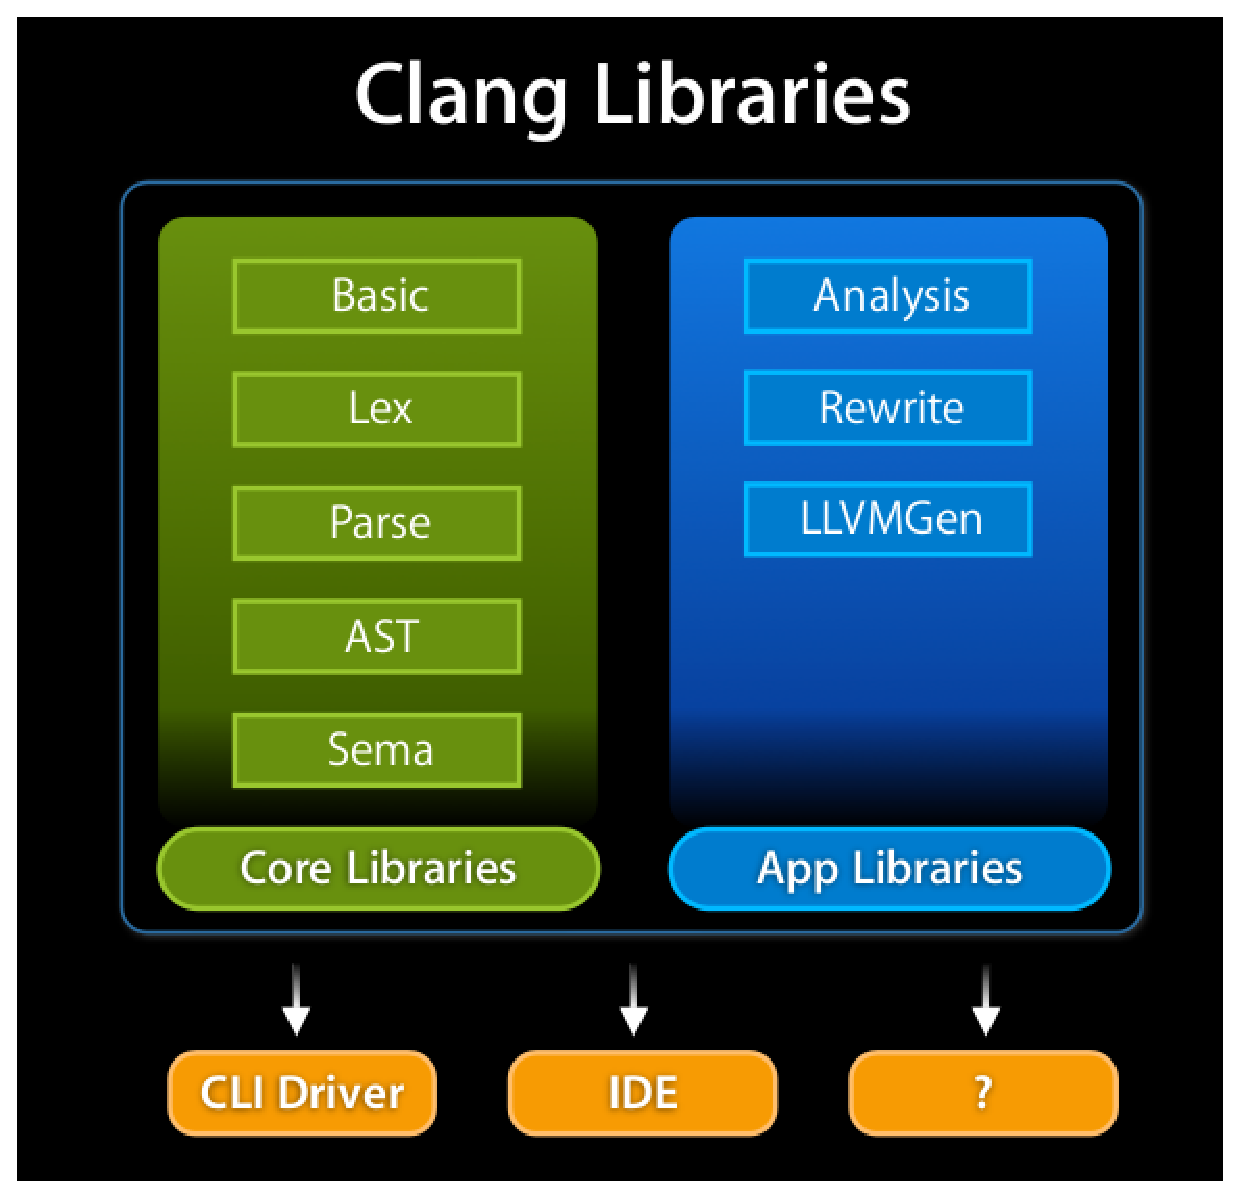
\includegraphics[width=0.4\textwidth]
      {figuras/clang_arch.eps}
      \caption{Arquitetura da ferramenta \emph{Clang}}
  \label{clang_arch}
\end{figure}

\subsubsection{\textit{Scripts} para análise estatística} \label{scripts}

Os \textit{scripts}\footnote{Disponível em:
\url{https://gitlab.com/paulormm/tese}} foram escritos utilizando linguagem R
\footnote{Informações em: \url{http://www.r-project.org/}} que foram
inicialmente desenvolvidos em \emph{Meirelles} (\citeyear{meirelles2013}). Foi escolhida a linguagem R
devido o seu foco e poder para a realização de análises estatísticas. Uma das
atividades desse processo de análise estatística que será realizado
por esses \textit{scripts} tentará identificar qual distribuição estatística melhor se encaixa nos dados referentes a 
determinada métrica, são utilizadas as seguintes distribuições estatísticas:

\begin{itemize}
  \item Pareto
  \item Pareto tipo 2
  \item Exponencial
  \item Gama
  \item Weibull
  \item Poison
\end{itemize}

Caso nenhuma das distribuições apresentadas consigam refletir os valores de uma determinada métrica, os
\textit{scripts} tentarão encontrar uma distribuição estatística que melhor se adeque. Gráficos de cada distribuição serão
gerados como saída desse processo de análise estatística, para melhor visualização dos dados. Como entrada teremos arquivos
CSV com os valores das métricas a serem analisadas.

Outro tipo de análise que poderá ser feita com essa suíte de \textit{scripts} será relacionada aos percentis das métricas.
Dada uma amostra (ou coleção de dados), os percentis são medidas que dividem a amostra ordenada (por ordem crescente dos dados) 
em cem (100) partes, cada uma com uma percentagem de dados aproximadamente igual. Define-se percentil k, ${Q_k}$, 
k recebendo valores de um (1) a noventa e nove (99), como sendo o valor tal que k\% dos elementos da amostra são menores ou 
iguais a ${Q_k}$ e os restantes (100-k)\% elementos da amostra são maiores ou iguais a ${Q_k}$ \cite{martins2013}. Os valores
de percentis utilizados são: 

\begin{multicols}{3}
  \begin{itemize}
    \item 1\%
    \item 5\%
    \item 10\%
    \item 25\%
    \item 50\%
    \item 75\%
    \item 90\%
    \item 95\%
    \item 99\%
  \end{itemize}
\end{multicols}

No processo do cálculo dos percentis o maior e menor valores são descartados, a
fim de remover \textit{outliers}, sendo \textit{outlier} um número que é muito maior 
ou menor que o resto dos números em uma dada série de números, segundo \emph{Hawkins}
(\citeyear{hawkins80}). A saída desse processo de análise estatística serão gráficos 
dos percentis e um arquivo texto com a quantidade de valores dentro de cada intervalo 
de percentil.

Tendo os percentis das métricas será possível fazer uma análise, sabendo em quais faixas geralmente ocorre 
determinados tipos de métricas, e tentar definir em qual faixa é aceitável ou não os valores das métricas de 
código fonte trabalhadas.

Foram desenvolvidos para este trabalho \textit{scripts}\footnote{Disponível em
\url{https://github.com/lucaskanashiro/clang\_parser\_html\_to\_csv}} para a adequação dos
dados advindos da ferramenta de extração de métricas de vulnerabilidade de
código fonte (\emph{Clang}, apresentado na subseção \ref{clang}). A saída padrão
da ferramenta é um arquivo HTML e a suíte de \textit{scripts} apresentados
anteriormente tem como um dos requisitos o arquivo de entrada ser do formato
CSV. Esses \textit{scripts} de adequação do formato dos dados utiliza-se de
expressões regulares para encontrar padrões e contar as ocorrências de
determinada cenário de vulnerabilidade. Com isso esses valores são escritos em
um arquivo CSV.

\subsection{Teste das Hipóteses} \label{subsec:teste_hipotese}

Nesta seção será feito o teste das hipóteses apresentadas na subseção
\ref{subsec:hipoteses}, utilizando as ferramentas apresentadas em \ref{subsec:ferramentas}.

\subsubsection{Coleta de Dados}

Para realizar a coleta dos dados e iniciar o teste das hipóteses, foram
feitas as seguintes atividades do processo descrito pelo fluxograma
\ref{fig:processo_estudo_de_caso}:

\begin{itemize}
  \item Selecionar projeto
  \item Obter código fonte
  \item Identificar como construir projeto
  \item Extrair métricas de vulnerabilidade
\end{itemize}

Para o teste dessas hipóteses foi selecionado um projeto de software considerado
representativo no contexto de vulnerabilidades de código fonte, que é o projeto
\emph{Linux Kernel}. Ele é a base para a grande maioria dos sistemas operacionais
disponíveis, esses sistemas são bastante utilizados por Engenheiros para
o próprio desenvolvimento de software, além de ser o sistema operacional em
execução na grande maioria dos servidores de aplicações, onde geralmente
atacantes exploram vulnerabilidades ao utilizarem-se de \textit{exploits}, como
foi apresentado na seção \ref{cap:metricas_vuln}.

O código fonte do projeto \emph{Linux Kernel} foi obtido no repositório \footnote{Disponível em:
\url{git://git.kernel.org/pub/scm/linux/kernel/git/torvalds/linux.git}} do seu
criador Linus Torvalds. Para encontrar o repositório foi utilizado a ferramenta
\emph{OpenHub} \footnote{Acessível em: \url{https://www.openhub.net/}}, onde
pode-se encontrar várias informações dessa natureza.

Para a construção (\textit{build}) do projeto existe documentação em diversos
locais, praticamente todas as distribuições \emph{Linux} possuem essa
documentação. Para este estudo de caso foi utilizada a documentação de uma das
distribuições \emph{Linux} mais conhecidas, do Ubuntu \footnote{Documentação para
  contrução do \emph{Linux Kernel}:
\url{https://help.ubuntu.com/community/Kernel/Compile}}.

Para a extração dos valores das métricas de vulnerabilidade de código fonte foi
utilizada a ferramenta \emph{Clang}, descrita na subseção
\ref{clang}. Foi utilizado a biblioteca de aplicativo
\textit{Analysis}, como apresentado na subseção já mencionada, mais conhecido como \emph{Clang Static
Analyzer}. Foi utilizado a documentação do próprio \emph{Clang Static Analyzer}
\footnote{Acessível em: \url{http://clang-analyzer.llvm.org/scan-build.html}},
entretanto, só é necessário adicionar uma chamada para a aplicação
(\textit{scan-build}) antes da linha de comando de construção do projeto.

Após a execução do \emph{Clang Static Analyzer} juntamente com a construção do
projeto, é dado um arquivo HTML como saída da aplicação. Como foi explicado na
subseção \ref{scripts}, esse não é o formato esperado pela suíte de
\textit{scripts} utilizados para análise estatística, com isso, foi feita a
adequação desses dados de maneira automatizada, como explicado no final da
subseção \ref{scripts}. Ao final, um arquivo CSV foi gerado com as métricas de
vulnerabilidade de código fonte por módulo do \emph{Linux Kernel}.

\subsubsection{Análise dos Resultados}

Tendo o arquivo CSV com a valoração das métricas de vulnerabilidade de código
fonte do projeto \emph{Linux Kernel}, houve a necessidade de uma reflexão antes
de prosseguir com o processo apresentado. Ao
fazer uma análise inicial dos valores das métricas, viu-se que grande parte
possuía valoração nula (igual a zero), representando que na maioria dos módulos
do \emph{Linux Kernel} não possuía vulnerabilidades de código fonte. Das vinte
métricas de vulnerabilidade de código fonte apresentadas na seção
\ref{cap:metricas_vuln}, apenas três delas possuíram valoração não nula em pelo
menos um dos módulos, sendo elas DNP, DUPV e SAIGV. 

Com isso, antes de se concluir o estudo de caso, já foi
possível negar a hipótese \emph{H1} e \emph{H2} apresentadas na subseção
\ref{subsec:hipoteses}, pois a forma de observar as métricas de vulnerabilidade
é diferente da de \textit{design} de código fonte, além da média dos valores
das métricas dos módulos não ser relevante para o seu acompanhamento. Métricas de \textit{design},
em geral, não possuem essa grande quantidade de valoração nula das métricas nos
módulos de um grande projeto como o \emph{Linux Kernel}, diferente do que
pode-se observar com as métricas de vulnerabilidade de código fonte. E como
grande parte dos módulos possui valoração das métricas nulas, a média desses
valores não é representativo para o acompanhamento das mesmas.

Após essa constatação, continuou-se o processo apresentado no fluxograma 
\ref{fig:processo_estudo_de_caso}. Foram realizadas as seguintes atividades:

\begin{itemize}
  \item Realizar análise estatística
  \item Analisar resultados
  \item Realizar conclusões
\end{itemize}

Antes de iniciar a atividade de análise estatística decidiu-se não testar a
hipótese \emph{H3} referente as distribuições estatísticas, pois, devido a
hipótese \emph{H1} ter sido negada, preferiu-se realizar uma análise qualitativa
antes para tentar entender como que deve-se observar métricas de vulnerabilidade de código
fonte antes de tentar encontrar distribuições estatísticas que represente-as.
Talvez, a distribuição estatística não seja relevante para acompanha-las, por
isso essa hipótese não foi testada neste estudo de caso.

Apesar de todas as hipóteses terem se esgotado nesse ponto do estudo de caso,
foi preferível a continuação do mesmo para tentar extrair alguma informação
útil no que se refere a questão do acompanhamento de métricas de vulnerabilidade de código
fonte.

Na atividade de realizar a análise estatística foi utilizada a suíte de
\textit{scripts} apresentados na subseção \ref{scripts}, entretanto, só foi
trabalhado com os percentis dos valores das métricas, a fim de tentar extrair
alguma informação relevante. Os gráficos dos percentis de cada uma das métricas 
de vulnerabilidade trabalhadas podem ser encontrados no apêndice \ref{anex:percentis}. 
A tabela \ref{tab:percentis} apresenta os valores dos percentis referentes a cada
uma das métricas de vulnerabilidade de código fonte gerados a partir da atividade
de análise estatística.

\begin{table}[h]
\resizebox{\textwidth}{!} & \textbf{5\%} & \textbf{10\%} & \textbf{25\%} & \textbf{50\%} & \textbf{75\%} & \textbf{90\%} & \textbf{95\%} & \textbf{99\%} & \textbf{Máximo} \\ \hline
\rowcolor[HTML]{EFEFEF} 
\textbf{AN}      & 0               & 0            & 0            & 0             & 0             & 0             & 0             & 0             & 0             & 0             & 0               \\ \hline
\textbf{ASOM}    & 0               & 0            & 0            & 0             & 0             & 0             & 0             & 0             & 0             & 0             & 0               \\ \hline
\rowcolor[HTML]{EFEFEF} 
\textbf{AUV}     & 0               & 0            & 0            & 0             & 0             & 0             & 0             & 0             & 0             & 0             & 0               \\ \hline
\textbf{BD}      & 0               & 0            & 0            & 0             & 0             & 0             & 0             & 0             & 0             & 0             & 0               \\ \hline
\rowcolor[HTML]{EFEFEF} 
\textbf{BF}      & 0               & 0            & 0            & 0             & 0             & 0             & 0             & 0             & 0             & 0             & 0               \\ \hline
\textbf{DBZ}     & 0               & 0            & 0            & 0             & 0             & 0             & 0             & 0             & 0             & 0             & 0               \\ \hline
\rowcolor[HTML]{EFEFEF} 
\textbf{DF}      & 0               & 0            & 0            & 0             & 0             & 0             & 0             & 0             & 0             & 0             & 0               \\ \hline
\textbf{DNP}     & 0               & 0            & 0            & 0             & 0             & 1             & 1,75          & 2             & 2,75          & 11,1499       & 17              \\ \hline
\rowcolor[HTML]{EFEFEF} 
\textbf{DUPV}    & 0               & 0            & 0            & 0             & 0             & 0             & 0             & 0             & 0             & 1,3499        & 2               \\ \hline
\textbf{FGBO}    & 0               & 0            & 0            & 0             & 0             & 0             & 0             & 0             & 0             & 0             & 0               \\ \hline
\rowcolor[HTML]{EFEFEF} 
\textbf{MLK}     & 0               & 0            & 0            & 0             & 0             & 0             & 0             & 0             & 0             & 0             & 0               \\ \hline
\textbf{OBAA}    & 0               & 0            & 0            & 0             & 0             & 0             & 0             & 0             & 0             & 0             & 0               \\ \hline
\rowcolor[HTML]{EFEFEF} 
\textbf{OSF}     & 0               & 0            & 0            & 0             & 0             & 0             & 0             & 0             & 0             & 0             & 0               \\ \hline
\textbf{PITFC}   & 0               & 0            & 0            & 0             & 0             & 0             & 0             & 0             & 0             & 0             & 0               \\ \hline
\rowcolor[HTML]{EFEFEF} 
\textbf{ROGU}    & 0               & 0            & 0            & 0             & 0             & 0             & 0             & 0             & 0             & 0             & 0               \\ \hline
\textbf{RSVA}    & 0               & 0            & 0            & 0             & 0             & 0             & 0             & 0             & 0             & 0             & 0               \\ \hline
\rowcolor[HTML]{EFEFEF} 
\textbf{SAIGV}   & 0               & 0            & 0            & 0             & 0             & 0             & 0             & 0             & 0             & 0             & 0               \\ \hline
\textbf{UA}      & 0               & 0            & 0            & 0             & 0             & 0             & 0             & 0             & 0             & 0             & 0               \\ \hline
\rowcolor[HTML]{EFEFEF} 
\textbf{UAF}     & 0               & 0            & 0            & 0             & 0             & 0             & 0             & 0             & 0             & 0             & 0               \\ \hline
\textbf{UAV}     & 0               & 0            & 0            & 0             & 0             & 0             & 0             & 0             & 0             & 0             & 0               \\ \hline
\end{tabular}
}
\caption{Percentis das métricas de vulnerabilidade extraídas do projeto \emph{Linux Kernel}}
\label{tab:percentis}
\end{table}

Analisando os resultados através dos gráficos gerados e a tabela \ref{tab:percentis}, 
pode-se ver que a maioria das métricas se manteve
em zero em todos os módulos do \emph{Linux Kernel}, tendo variado apenas os
valores das métricas DNP (\ref{graphic:dnp}) e DUPV (\ref{graphic:dupv}). O
gráfico da métrica SAIGV também é uma reta em zero, apesar de ter apenas uma ocorrência
não nula, devido a exclusão do menor e maior valor no processo de análise
estatística. Levando em consideração apenas os gráficos das métricas não nulas, 
pode-se ver que os valores das métricas se concentram nos percentis mais elevados, 
com isso, conclui-se, que a grande maioria dos valores dessas métricas possuem valores similares na
maioria dos módulos, não variando muito a sua valoração. Entretanto, essa
informação não agrega tanto valor no que diz respeito a como se acompanhar
métricas de vulnerabilidade de código fonte em um projeto de software, apenas nos mostra que a
maioria dos valores das métricas são similares, ou seja, se o valor de uma
métrica variar muito de um módulo para outro, existe um indício de que algo pode
estar errado.

Ao realizar a análise apresentada acima, chegou-se a conclusão que para entender
melhor as métricas de vulnerabilidade de código fonte é necessário realizar uma
análise qualitativa ao invés de quantitativa. Com isso, resolveu-se realizar uma
nova análise, agora qualitativa, das métricas de vulnerabilidade de código fonte, 
para tentar compreender um pouco melhor a natureza dessas métricas, essa análise 
é apresentada na seção \ref{sec:analise_qualitativa}.

\section{Análise Qualitativa} \label{sec:analise_qualitativa}

Nesta seção será apresentada uma análise qualitativa das métricas de vulnerabilidade 
de código fonte. Para iniciar essa análise em um perspectiva diferente da que foi 
apresentada na seção \ref{subsec:teste_hipotese}, identificou-se a necessidade de informações
de uma maior quantidade de projetos de software, além do projeto \emph{Linux Kernel} que foi
utilizado no estudo de caso apresentado. Foram selecionados alguns projetos de naturezas
diferentes, respeitando os únicos requisitos de possuir a linguagem de programação C/C++ como
base da sua implementação e ser um software livre, sendo eles:

\begin{multicols}{2}
\begin{itemize}
  \item Bash
  \item Blender
  \item FFmpeg
  \item Firefox
  \item Gstreamer
  \item Inetutils
  \item OpenSSH
  \item OpenSSL
  \item Python2.7
  \item Ruby-2.1
\end{itemize}
\end{multicols}

Considerou-se que talvez a inserção de projetos de software com propósitos diferentes
pudesse agregar algum tipo de informação interessante para a interpretação e acompanhamento
das métricas de vulnerabilidade de código fonte. Onde uma possível hipótese seria que os
valores das métricas de vulnerabilidade variam de maneira diferente dependendo da natureza 
do software.

O processo realizado com cada um desses projetos foi similar ao aplicado no estudo de caso
para coleta de dados, apresentada na subseção \ref{subsec:teste_hipotese}, com o projeto 
\emph{Linux Kernel}. Após feita a coleta de dados, havia disponível um arquivo CSV para
cada projeto contendo as métricas de vulnerabilidade de código fonte por módulo. Ao invés
de prosseguir com o processo realizado no estudo de caso, onde nesta etapa seria feita uma
análise estatística quantitativa dos valores das métricas, o problema foi abordado de 
maneira diferente, como será apresentado a seguir.

Levando em conta que nesta fase as métricas de vulnerabilidade de código fonte já estavam
disponíveis, as atividades realizadas nesta análise qualitativa foram as seguintes:

\begin{enumerate}
  \item Contabilizar quantidade total de módulos presentes no projeto a ser analisado.
  \item Selecionar métricas de vulnerabilidade com valoração não nula para o projeto em questão.
  \item Contabilizar quantidade de módulos afetados por cada uma das métricas anteriormente selecionadas.
  \item Calcular porcentagem de módulos do projeto afetados por alguma vulnerabilidade.
  \item Calcular porcentagem de módulos do projeto afetados por cada uma das vulnerabilidades 
    referentes as métricas selecionadas.
  \item Analisar os resultados obtidos.
\end{enumerate}

Essas atividades foram definidas e realizadas no decorrer de um processo empírico, a fim de melhor
entender o referido problema. A seguir, serão apresentados os resultados obtidos a partir da nova
abordagem de análise.

A tabela \ref{tab:modulos_proj} apresenta uma visão geral de cada projeto aqui analisado, contendo
informações como número total de módulos C/C++ do projeto, número total de módulos que sofrem
algum tipo de vulnerabilidade e porcentagem dos módulos do projeto vulneráveis.

\begin{table}[h]
\resizebox{\textwidth}{!}{%
\begin{tabular}{cccc}
\hline
\textbf{Projeto}      & \textbf{Nº total de Módulos} & \textbf{Nº total de Módulos vulneráveis} & \textbf{\% de Módulos vulneráveis} \\ \hline
\rowcolor[HTML]{EFEFEF} 
\textbf{Bash}         & 253                          & 36                                       & 14.2292                            \\ \hline
\textbf{Blender}      & 1472                         & 106                                      & 7.2010                             \\ \hline
\rowcolor[HTML]{EFEFEF} 
\textbf{FFmpeg}       & 1776                         & 100                                      & 5.6306                             \\ \hline
\textbf{Firefox}      & 12404                        & 328                                      & 2.6443                             \\ \hline
\rowcolor[HTML]{EFEFEF} 
\textbf{Gstreamer}    & 264                          & 22                                       & 8.3333                             \\ \hline
\textbf{Inetutils}    & 2576                         & 27                                       & 1.0481                             \\ \hline
\rowcolor[HTML]{EFEFEF} 
\textbf{Linux Kernel} & 23056                        & 43                                       & 0.1865                             \\ \hline
\textbf{OpenSSH}      & 248                          & 14                                       & 5.6451                             \\ \hline
\rowcolor[HTML]{EFEFEF} 
\textbf{OpenSSL}      & 974                          & 26                                       & 2.6694                             \\ \hline
\textbf{Python2.7}    & 551                          & 32                                       & 5.8076                             \\ \hline
\rowcolor[HTML]{EFEFEF} 
\textbf{Ruby-2.1}     & 381                          & 20                                       & 5.2493                             \\ \hline
\end{tabular}
}
\caption{Análise de Módulos por Projeto}
\label{tab:modulos_proj}
\end{table}

Analisando os dados apresentados acima pode-se perceber que, em média, cinco porcento (5\%) dos módulos
dos projetos são de alguma forma vulneráveis devido a erros de codificação. Os valores absolutos da
quantidade de módulos afetados são bem inferiores ao de módulos totais, o que explica a grande quantidade
de valores nulos de métricas de vulnerabilidades em grande parte dos módulos de um projeto.

Pode-se perceber que alguns projetos com propósito similar, como o \emph{Python2.7} e o \emph{Ruby-2.1}
que são linguagens de programação, possuem valores bem próximos de módulos vulneráveis, o que pode ser um
indício de que a hipótese levantada no início desta seção seja verdadeira, onde projetos com propósitos
similares se comportam de maneira parecida.

Além disso, os projetos com maiores taxas de módulos vulneráveis, em geral, são projetos que não possuem
um forte viés em segurança, como o \emph{Blender} e \emph{Gstreamer}. A exceção nesse caso seria o \emph{Bash},
pois o mesmo possui uma alta porcentagem de módulos vulneráveis, entretanto, é um alvo constante de ataques e
deveria se preocupar em não deixar brechas de segurança para atacantes. Isso mostra que o \emph{Bash} por 
enquanto ainda é uma boa opção para a utilização de \textit{exploits} por parte de atacantes.

Durante esta análise foram identificados um conjunto de métricas de vulnerabilidade que são mais comuns e
ocorrem com mais frequência. A métrica de vulnerabilidade mais frequente nos projetos analisados foi a DNP,
a mesma está presente em todos os projetos. Além de ser frequente entre os projetos, essa métrica também
é comum a boa parte dos módulos de um mesmo projeto. Na tabela \ref{tab:dnp} é apresentado a quantidade
absoluta de módulos que possuem o cenário de vulnerabilidade de desreferência de ponteiro nulo e a porcentagem
de módulos que a mesma atinge de cada projeto.


\begin{table}[h]
\resizebox{\textwidth}{!}{%
\begin{tabular}{cccc}
\hline
\textbf{Projeto}      & \textbf{Nº total de Módulos} & \textbf{Nº total de Módulos vulneráveis} & \textbf{\% de Módulos vulneráveis} \\ \hline
\rowcolor[HTML]{EFEFEF} 
\textbf{Bash}         & 253                          & 22                                       & 8.6956                             \\ \hline
\textbf{Blender}      & 1472                         & 93                                       & 6.3179                             \\ \hline
\rowcolor[HTML]{EFEFEF} 
\textbf{FFmpeg}       & 1776                         & 37                                       & 2.0833                             \\ \hline
\textbf{Firefox}      & 12404                        & 218                                      & 1.7574                             \\ \hline
\rowcolor[HTML]{EFEFEF} 
\textbf{Gstreamer}    & 264                          & 16                                       & 6.0606                             \\ \hline
\textbf{Inetutils}    & 2576                         & 6                                        & 0.2329                             \\ \hline
\rowcolor[HTML]{EFEFEF} 
\textbf{Linux Kernel} & 23056                        & 40                                       & 0.1734                             \\ \hline
\textbf{OpenSSH}      & 248                          & 7                                        & 2.8225                             \\ \hline
\rowcolor[HTML]{EFEFEF} 
\textbf{OpenSSL}      & 974                          & 14                                       & 1.4373                             \\ \hline
\textbf{Python2.7}    & 551                          & 18                                       & 3.2667                             \\ \hline
\rowcolor[HTML]{EFEFEF} 
\textbf{Ruby-2.1}     & 381                          & 10                                       & 2.6246                             \\ \hline
\end{tabular}
}
\caption{Métrica DNP por projeto}
\label{tab:dnp}
\end{table}


Fazendo um comparativo entre as tabelas \ref{tab:modulos_proj} e \ref{tab:dnp}, pode-se ver que na
maioria dos projetos o cenário de vulnerabilidade tratado pela métrica DNP é responsável pela maior
parte das vulnerabilidades, como por exemplo no projeto \emph{Linux Kernel}. O \emph{Linux Kernel}
é o projeto com menor taxa de módulos vulneráveis, sendo igual a 0.1865\%, logo, é o projeto mais 
seguro dentre os estudados. Ele possui quarenta e três (43) módulos vulneráveis e quarenta (40) deles
possuem o cenário referente a métrica DNP, ou seja, a DNP é responsável praticamente por 93.02\% das 
vulnerabilidades presentes no \emph{Linux Kernel}. Esse dado só foi apresentado para evidenciar que
essa vulnerabilidade deve ser acompanhada de perto, pois até projetos preocupados com essa questão
de segurança sofrem desse mal. No momento da implementação deve-se tomar cuidado para não acessar 
locais de memória que não foram alocados, ou seja, não acessar ponteiros nulos,
podendo utilizar-se de validações antes da chamada ao ponteiro.

A métrica de vulnerabilidade de código fonte DNP se apresenta como a mais
recorrente entre as aŕesentadas
no contexto deste trabalho, entretanto, outras métricas também aparecem com uma frequência um pouco menor,
como as métricas AN e ROGU. O resumo da frequência das métricas de vulnerabilidade de código fonte por módulo
de cada um dos projetos poderá ser visto no apêndice \ref{anex:analise_qualitativa}. A seguir uma lista com
as mais recorrentes métricas de vulnerabilidade de código fonte identificadas:

\begin{multicols}{2}
\begin{itemize}
  \item DNP
  \item AN
  \item ROGU
  \item AUV
\end{itemize}
\end{multicols}

Esta análise qualitativa apresentou-se mais produtiva para um entendimento inicial do comportamento
das métricas de vulnerabilidade de código fonte do que uma análise quantitativa. Com essa análise foi
possível levantar uma nova hipótese a ser testada, onde projetos com propósitos
semelhantes se comportam de 
maneira similar, além de determinar um conjunto de métricas de vulnerabilidade mais recorrentes, que devem
ser acompanhadas mais de perto em um projeto de software.

